\chapter{Results}

This chapter presents the results of the analysis performed using the framework. Keep in mind that POX isn't designed to compete with the very best (cite POX's own graphs showing it's worse than NOX), but is designed for academia. Given that, none of this will be compared with existing industry-standard controllers such as Beacon or OpenDaylight (what is with all the light metaphors?).

Also all testing will be done entirely in software, no real switches will be used.

\section{Comparison of Routing Metrics}
Analysis goes here. dunno what to call this, routing performance or whatever. something title-capsy.

\begin{figure}
\centering
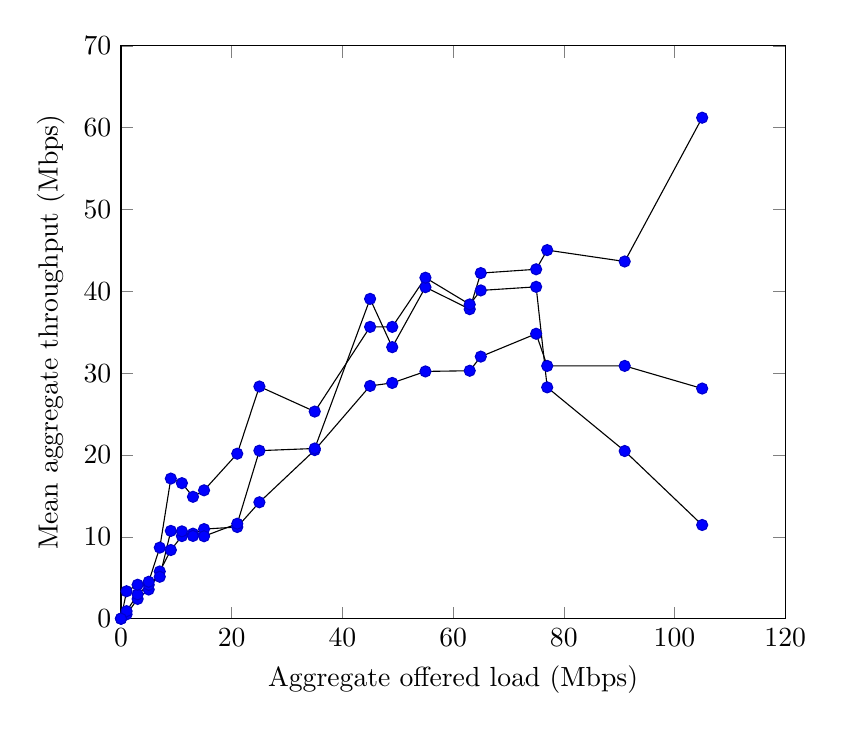
\begin{tikzpicture}
  \begin{axis}[
    xlabel = Aggregate offered load (Mbps),
    ylabel = Mean aggregate throughput (Mbps),
    xmin=0, xmax=120, ymin=0, ymax=70,
    scale only axis
  ]

  \addplot[scatter, scatter src=\thisrow{class},
      error bars/.cd, y dir=both, x dir=both, y explicit, x explicit, error bar style={draw=none}]
      table[x=x,y=y,x error=xerr,y error=yerr] {
    x       xerr    y        yerr       class
    0 0 0 0 0
    1 0 0.5233626 0 0
    3 0 2.4087152 0 0
    5 0 3.5592573 0 0
    7 0 5.762373  0 0
    9 0 8.3855359 0 0
    11  0 10.0891018  0 0
    13  0 10.3842113  0 0
    15  0 10.9418756  0 0
    21  0 11.196595 0 0
    25  0 14.220054 0 0
    35  0 20.597453 0 0
    45  0 28.4402179  0 0
    49  0 28.8025593  0 0
    55  0 30.2096573  0 0
    63  0 30.2932245  0 0
    65  0 32.0205427  0 0
    75  0 34.8129119  0 0
    77  0 30.8807939  0 0
    91  0 30.8843334  0 0
    105 0 28.1190057  0 0
  };


  \addplot[scatter, scatter src=\thisrow{class},
      error bars/.cd, y dir=both, x dir=both, y explicit, x explicit, error bar style={draw=none}]
      table[x=x,y=y,x error=xerr,y error=yerr] {
    x       xerr    y        yerr       class
    0 0 0 0 0
    1 0 0.911334  0 0
    3 0 2.968354  0 0
    5 0 4.13075065  0 0
    7 0 5.1164835 0 0
    9 0 10.7210935  0 0
    11  0 10.6638835  0 0
    13  0 10.108582 0 0
    15  0 10.0703918  0 0
    21  0 11.6003224  0 0
    25  0 20.527074 0 0
    35  0 20.793514 0 0
    45  0 39.074855 0 0
    49  0 33.1735586  0 0
    55  0 40.50877  0 0
    63  0 37.815874 0 0
    65  0 42.2256273  0 0
    75  0 42.691425 0 0
    77  0 45.0346897  0 0
    91  0 43.6423792  0 0
    105 0 61.2153794  0 0
  };


  \addplot[scatter, scatter src=\thisrow{class},
      error bars/.cd, y dir=both, x dir=both, y explicit, x explicit, error bar style={draw=none}]
      table[x=x,y=y,x error=xerr,y error=yerr] {
    x       xerr    y        yerr       class
    0 0 0 0 0
    1 0 3.34752325  0 0
    3 0 4.14193875  0 0
    5 0 4.504648  0 0
    7 0 8.68050385  0 0
    9 0 17.1164394  0 0
    11  0 16.555942725  0 0
    13  0 14.88846265 0 0
    15  0 15.6809798  0 0
    21  0 20.1572935  0 0
    25  0 28.3662994  0 0
    35  0 25.3032905  0 0
    45  0 35.652433425  0 0
    49  0 35.651522775  0 0
    55  0 41.6621008  0 0
    63  0 38.4004853  0 0
    65  0 40.1076881  0 0
    75  0 40.547581725  0 0
    77  0 28.262232875  0 0
    91  0 20.482859125  0 0
    105 0 11.444907875  0 0
  };

  \end{axis}
\end{tikzpicture}
\caption{A great graph}
\label{fig:graph}
\end{figure}

\begin{table}
\caption{Summary of incredible achievements}
\end{table}

\section{Scalability of Objective Functions}
The results sure were great.
well. they were pretty much as expected. discuss them i guess.
stats-gathering is really hard and it is sensitive to it. i think some people thought
about it but it's worth a whole thesis on its own really.
somewhat limited by not being able to discover link capacities (whatshisname is
doing his thesis on it so it’s a separate/big problem). meant had to use topos with
constant capacities and in practical terms identical capacities. considered writing a
thing to let you fake the topo too but w/ever.

These graphs only show the results of experiments on a certain class of topologies: ones with constant and therefore symmetrical link capacities. This was discussed earlier in section SECTION.


Running experiments on Mininet means that there are practical limitations of the system which limit the size of networks which can be emulated with Mininet; this limit is hit long before the scalability of objective functions becomes a factor. However, it is possible to test the scalability of individual objective functions without the surrounding framework, by passing mock network graphs and flow statistics to the function. 

The Al-Fares fat-tree is parametrisable by a parameter k, which indicates the number of ports per commodity switch used in the network; this produces a network with f(k) = SOMETHING switches and g(k) = SOMETHINGELSE hosts in total, and is therefore easy to scale up to large networks for scalability testing. In this test, flows were randomly generated between 16 random hosts, for Al-Fares networks starting from k = 4 until further tests became impractically slow to run (greater than X seconds).  The results of this testing are shown in figure FIGURE, for each of the three routing metrics under consideration.

As expected, the shortest-path metric scales extremely well. The basic algorithm is well-understood, and the particular implementation used here is the one provided with NetworkX, which includes a number of small optimisations as well.

The residual spare capacity implementation is based on the formulation described originally by Walkowiak. In his PAPER he gives the WHATEVER of the algorithm as O(crazy). As seen in section SECTION, the performance of the algorithm as a whole depends mostly on the number of possible paths in the network: for every, this must be considered. In its original form, the solution becomes unworkably slow (greater than X seconds) at k = 6 or SOMETHING, with just X switches considered; this corresponds to Y possible paths for any given source/destination pair. One major optimisation was therefore implemented: the length of possible paths considered is limited to 6 hops. This is enough hops to allow multiple paths to each aggregation and core switch, but not to bounce indefinitely and unnecessarily between the core and aggregation and aggregation and edge layers. Figure FIGURE demonstrates how much the scalability of the RSC metric is dependent on the maximum path length considered.

The widest path metric performs quite poorly for such a well-known routing metric. The algorithm is based on a modified Dijkstra's algorithm, as described in section SECTION, which is not known to be particularly inefficient; the poor performance of the metric in these experiments is likely to be due to poor implementation. In particular, the algorithm must consider every path in the network, so, as for the RSC metric, the number of paths in an Al-Fares fat-tree can be very high and this is likely to be a significant factor in the algorithm's scalability. Unlike for RSC, however, limiting the number of paths considered was non-trivial due to the particular implementation, so this optimisation was not implemented. The dramatic effect of path length on the RSC metric seems to indicate that this would provide better scalability in this similar metric as well.

In this thesis, the objective function was only run once, the resulting throughput measured and the experiment stopped. Normally, the objective function would be run many times. It is quite impractical to try to globally optimise the entire network for every single new flow, and without letting the flow run for some time it is impossible to determine the demand, which is required to run the global optimisation anyway. In general, then, it seems that the approach used in this thesis would be reasonable: route flows initially along the shortest path, then every few seconds (as deemed appropriate; the gap would be shorter in a network mostly consisting of short bursts of traffic compared to large elephant flows) globally-optimal routes are recalculated.

In a normal scenario, however, the routing recalculation is performed every few seconds, and it is likely that many flows would be similar between calculations. This assumption can be made stronger if flows are consolidated; for example, group 'all HTTP traffic' along similar paths instead of calculating flow rules for individual 5-tuples, so that it is more likely that flows will average out to similar demands between calculations. In such an environment, recalculating the flow rules for the entire network from scratch becomes unreasonable. In many optimisation techniques, such as WHATEVER GLPK USES and simulated annealing as used in HEDERA, starting from an estimated solution which is close to the optimum greatly decreases the time taken to reach optimal levels; the previous calculation could be used as such an estimated solution. The implementation of this is non-trivial, and limits the use of third-party interfaces such as PuLP, since there is no way to specify a starting estimate for most solvers. Storing the state of, for example, the matrices used for linear algebra solutions to optimisation problems would be far more interesting. However, this is far outside the scope of this project and definitely in the realm of 'future work'.

From the perspective of this thesis, where the largest network considered was an Al-Fares fat-tree with k=4, the time taken to calculate routes is negligible for all routing metrics.


\section{Evaluation of Framework}

stuff about how great \thesis is
